\newpage

%   (III' $\cup$ II') $\cap$ (II' $\cap$ I)' - (IV' - III)
\textbf{f)} Analizando paso por paso el segundo inciso \ref{f}, se puede resolver en tres partes \textbf{} , \textbf{} y \textbf{} para así unir los tres subconjuntos \\

Resolviendo \textbf{(III' $\cup$ II')}

\begin{align*}
(III' \cup II')  &= \{ k, l, m, n, p, q, r, s, t, v, w, x, y, z \} \cup  \{ a, b, c, d, e, f, g, i, k, l, m, n, o, t, u, v, w, x, y, z \} \\
  &=   \{ a, b, c, d, e, f, g, i, k, l, m, n, o, p, q, r, s, t, u, v, w, x, y, z \}       \\
\end{align*}

Resolviendo \textbf{(II' $\cap$ I)' }

\begin{align*}
(II' \cap I)'   &= (\{ a, b, c, d, e, f, g, i, k, l, m, n, o, t, u, v, w, x, y, z \} \cap \{a, e, i, o, u\})' \\
  &=  ( \{a, e, i, o, u\} )' \\
  &= \{ b, c, d, f, g, h, j, k, l, m, n, p, q, r, s, t, v, w, x, y, z \}  \\
\end{align*}


Resolviendo \textbf{(IV' - III)}

\begin{align*}
(IV' - III)  &= \{ a, b, c, d, e, i, o, t, u, v, w, x, y, z \} - \{ a, b, c, d, e, f, g, h, i, j, o, u  \} \\
  &=  \{ t, v, w, x, y, z \}  \\
\end{align*}

Juntando los tres lados para armar (III' $\cup$ II') $\cap$ (II' $\cap$ I)' - (IV' - III):

\begin{align*}
(III' \cup II') \cap (II' \cap I)' - (IV' - III) &= \{ a, b, c, d, e, f, g, i, k, l, m, n, o, p, q, r, s, t, u, v, w, x, y, z \} \\ &\cap \{ b, c, d, f, g, h, j, k, l, m, n, p, q, r, s, t, v, w, x, y, z \}  - \{ t, v, w, x, y, z \}  \\
  &=  \{b, c, d,  f, g, k, l, m, n, p, q, r, s, t, v, w, x, y, z \} 
 - \{ t, v, w, x, y, z \} \\
 &=  \{  b, c, d, f, g, k, l, m, n, p, q, r, s      \} 
\end{align*}

Por lo tanto el resultado es:

\begin{equation*}
    \boxed{(III' \cup II') \cap (II' \cap I)' - (IV' - III)  =  \{  b, c, d, f, g, k, l, m, n, p, q, r, s      \}    }
\end{equation*}


\newpage


Para obtener el diagrama de Venn, se puede hacer por partes, el lado derecho y lado izquierdo, quedando: \\


\textbf{(III' $\cup$ II')}: 

\begin{figure}[htbp]
\centering
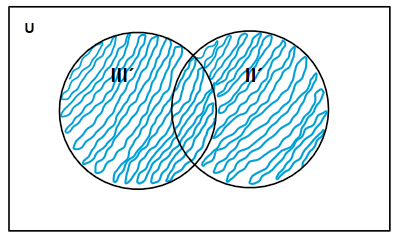
\includegraphics[width=8cm]{f/aa.png}
\caption[]{Diagrama de Venn de (III' $\cup$ II')}
\end{figure} 


\textbf{(II' $\cap$ I)'}:

\begin{figure}[htbp]
\centering
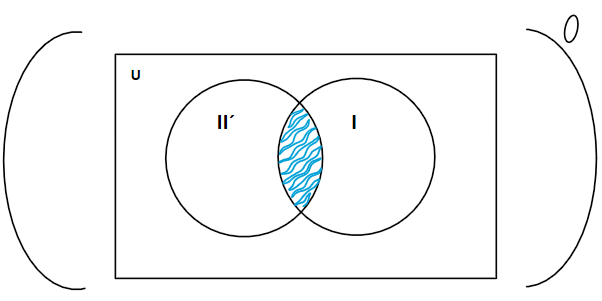
\includegraphics[width=8cm]{f/bb.png}
\caption[]{Diagrama de Venn de (II' $\cap$ I)'}
\end{figure} 

Sacando el complemento, queda el diagrama

\begin{figure}[htbp]
\centering
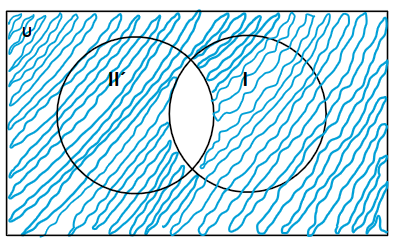
\includegraphics[width=8cm]{f/bbb.png}
\caption[]{Diagrama de Venn de (II' $\cap$ I)'}
\end{figure} 

\newpage

\textbf{(IV' - III)}:

\begin{figure}[htbp]
\centering
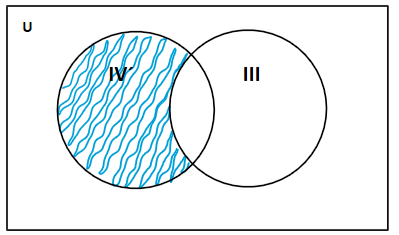
\includegraphics[width=7cm]{f/cc.png}
\caption[]{Diagrama de Venn de (IV' - III)}
\end{figure} 

Haciendo la intersección de (III' $\cup$ II') $\cap$ (II' $\cap$ I)', quedando así:

\begin{figure}[htbp]
\centering
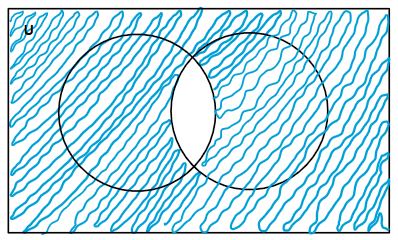
\includegraphics[width=7cm]{f/aabb.png}
\caption[]{Diagrama de Venn de (III' $\cup$ II') $\cap$ (II' $\cap$ I)'}
\end{figure} 


Haciendo la diferencia de (III' $\cup$ II') $\cap$ (II' $\cap$ I)' - (IV' - III), quedando así:

\begin{figure}[htbp]
\centering
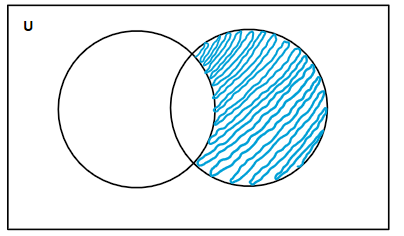
\includegraphics[width=7cm]{f/aabbcc.png}
\caption[]{Diagrama de Venn de (III' $\cup$ II') $\cap$ (II' $\cap$ I)' - (IV' - III)}
\end{figure} 